\documentclass[12pt]{article}
\usepackage[paper=letterpaper,margin=2cm]{geometry}
\usepackage{amsmath}
\usepackage{amssymb}
\usepackage{amsfonts}
\usepackage{newtxtext, newtxmath}
\usepackage{enumitem}
\usepackage{titling}
\usepackage[colorlinks=true]{hyperref}
\usepackage{graphicx}
\usepackage{csvsimple}
\usepackage{luacode}
\setlength{\droptitle}{-6em}

% Enter the specific assignment number and topic of that assignment below, and replace "Your Name" with your actual name.

\title{\textbf{COMP0078 Assignment 2}}
\author{Student Numbers: 21168615 \& 19004608 \\ }
\date{Dec 14, 2022}

\begin{document}
    \maketitle
\section{PART I}
\subsection{Kernel Perceptron}
\subsubsection{Experimental Results}

\begin{itemize}
    \item[1.] Basic Results:

    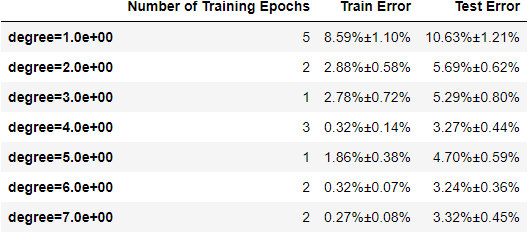
\includegraphics{outputs/part1/q1.png}


    \item[2.] Cross Validation Results:

    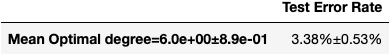
\includegraphics{outputs/part1/q2.png}

    \item[3.] Confusion Matrix:

    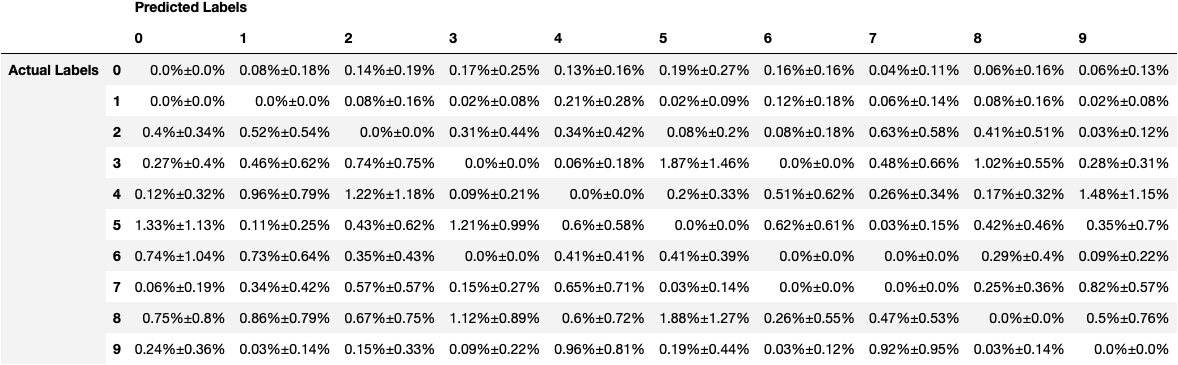
\includegraphics{outputs/part1/q3_confusion.png}
\newpage
    \item[4.] Hardest to predict images:

    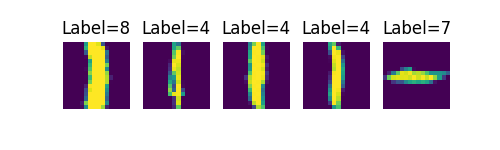
\includegraphics{outputs/part1/q4.png}
    \newpage
    \item[5.] Basic Results:

    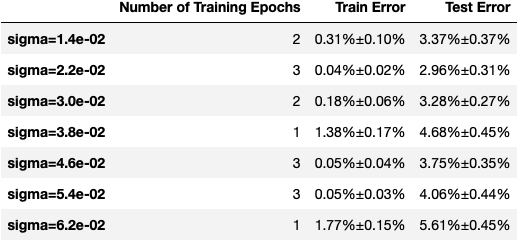
\includegraphics{outputs/part1/q5_1.png}

    Cross Validation Results:

    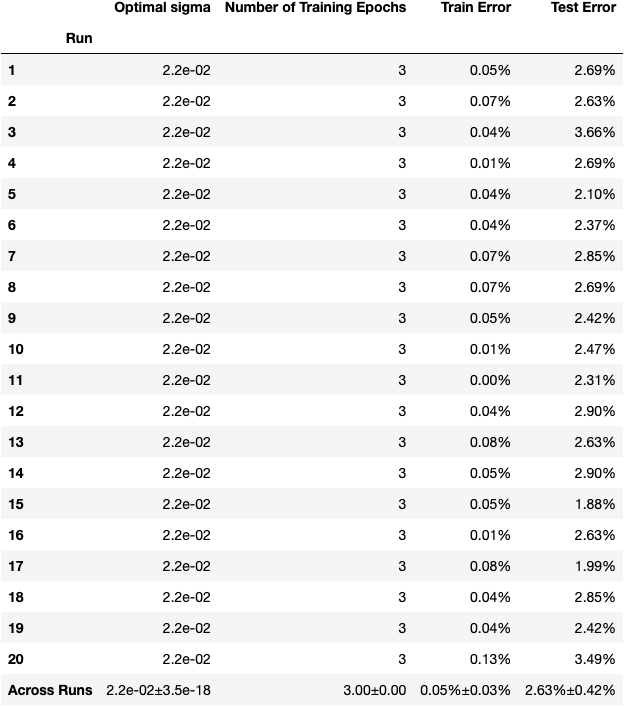
\includegraphics{outputs/part1/q5_2.png}
\end{itemize}
\subsubsection{Discussions}
    Choice of Parameters that weren't cross validated

    Generalisation to k-classifiers

    Kernel Comparison

    Kernel Perceptron Implementation


\newpage
\section{PART II}
\subsection{Semi-supervised Leanrning via Laplacian Interpolation}
Experimental report for the laplacian interpolation approach:
\\

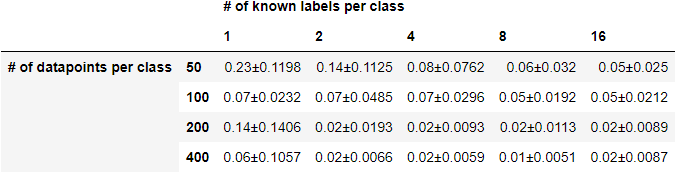
\includegraphics{outputs/part2/laplacian_interpolation_report.png}

\\

And for the laplacian kernel method:

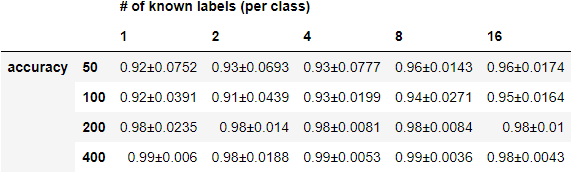
\includegraphics{outputs/part2/laplacian_kernel_interpolation_report.png}



\newpage



\section{PART III}
\subsection{Questions}
\begin{itemize}
    \item[1.]
    \item[2.]
    \item[3.]
\end{itemize}
\end{document}
